Cartographer is a real\hyp{}time \acs{slam} system that support \acs{2d} and \acs{3d} across multiple platforms and sensor configurations. Aswell as a build\hyp{}in \acs{ros} implementation. The system is developed and maintained by Google. \cite{cartographer_ros_integration}

The reason for researching this algorithm is that it is well maintained and often used in a lot of projects. The conclusion that Cartographer is not a real \acs{3d} but more a \acs{2.5d} algorithm came during the research. \acs{2.5d} is a pseudo\hyp{}\acs{3d} perspective. The algorithm can combine multiple \acs{2d} scans and combine them, but that is not truly \acs{3d}. \cite{liang2016generating}

\begin{figure}[!h]
  \centering
  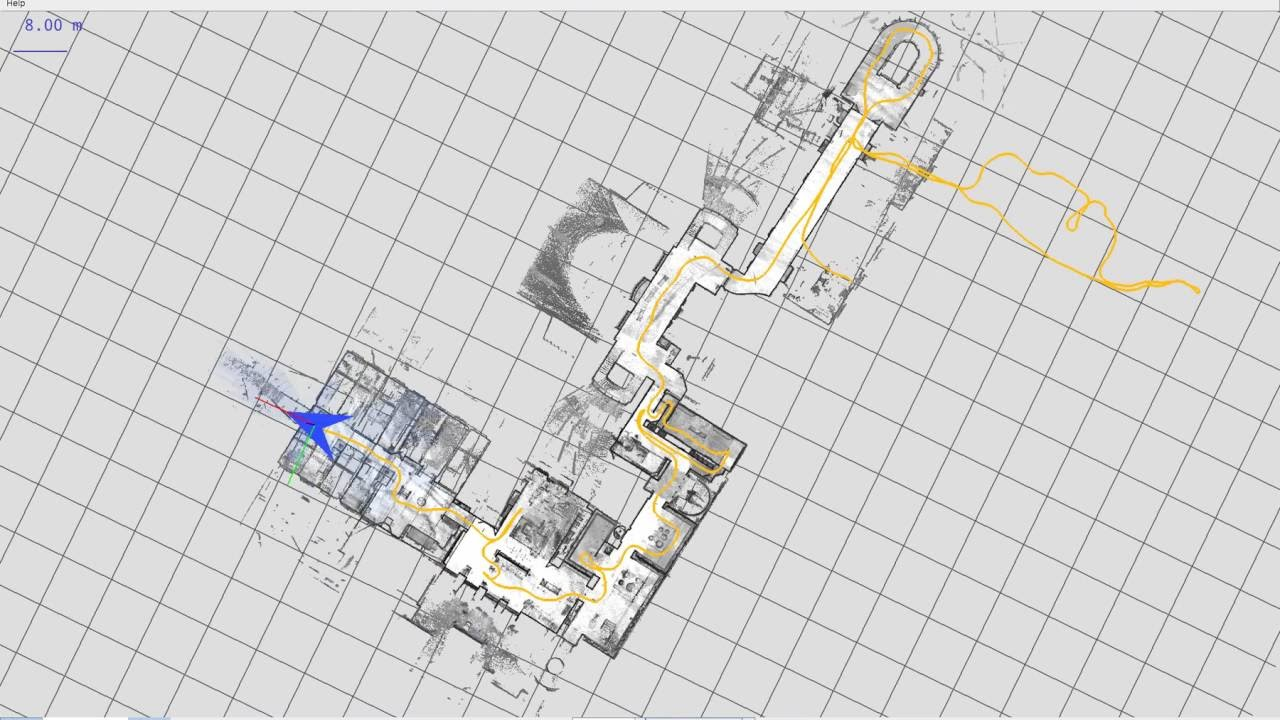
\includegraphics[width=0.75\linewidth]{images/cartographer_2d.jpg}
  \caption{Cartographer 2D example \cite{cartographer_google_open_source}}
\end{figure}

\begin{figure}[!h]
  \centering
  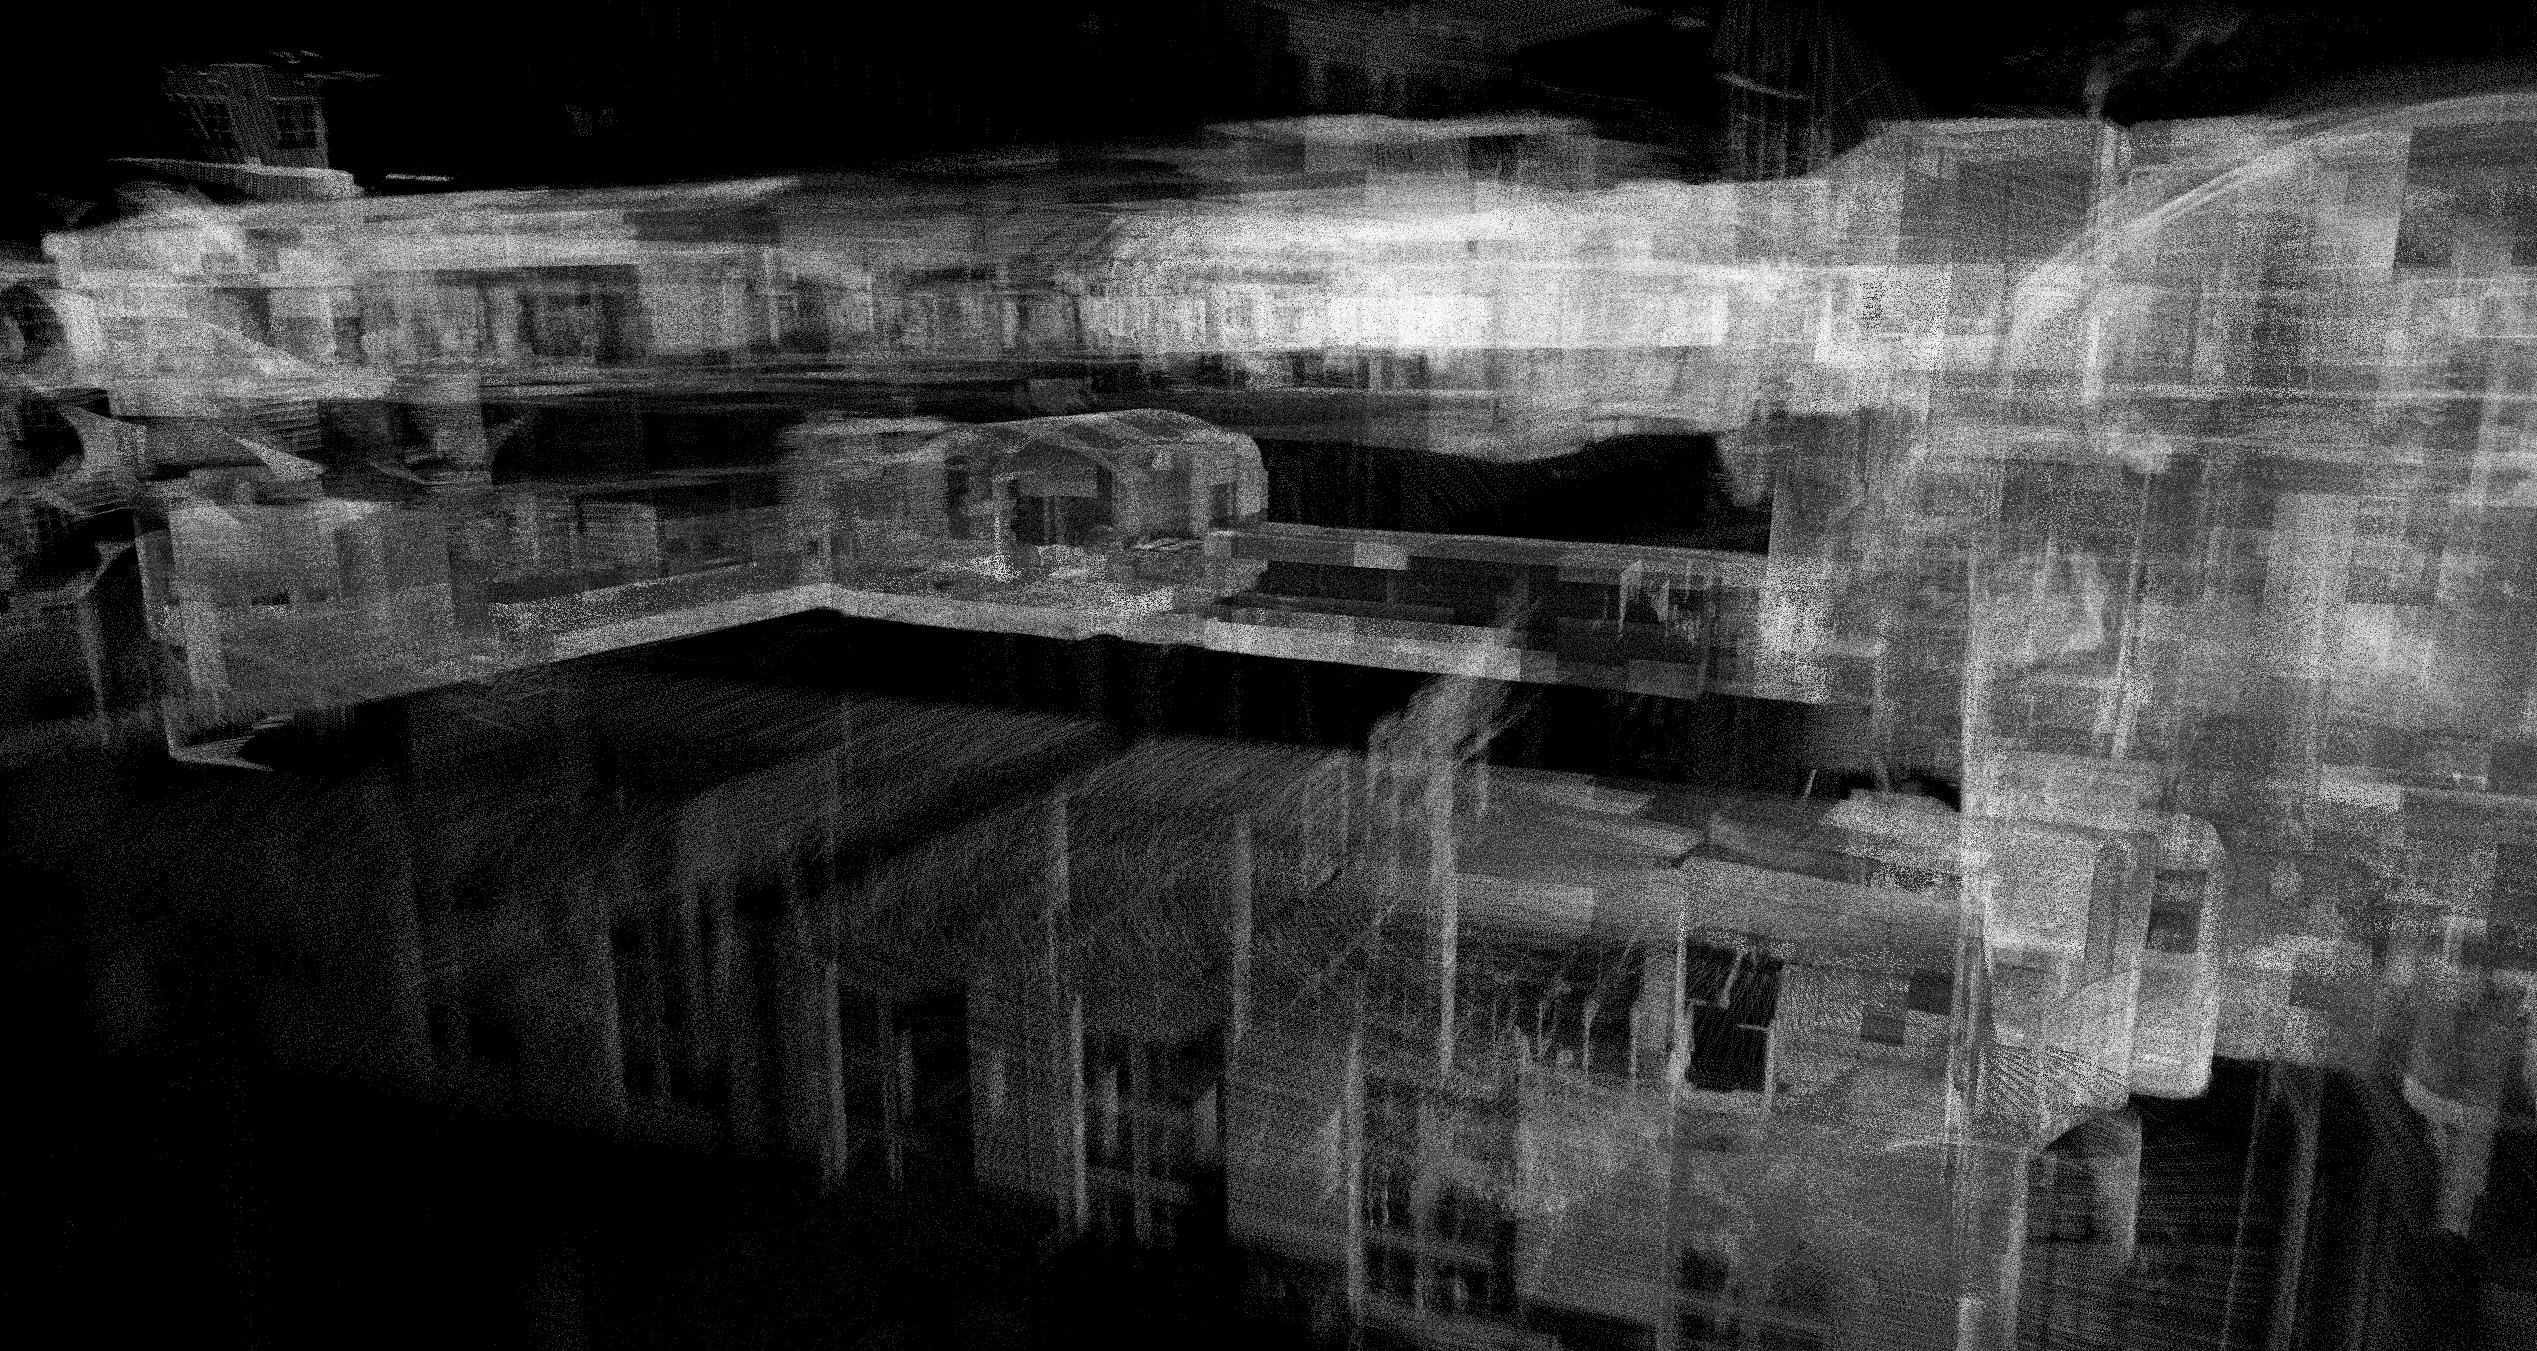
\includegraphics[width=0.75\linewidth]{images/cartographer_3d.jpg}
  \caption{Cartographer 3D example \cite{cartographer_exploiting_map}}
\end{figure}